\documentclass[12pt]{article}

\newcommand{\reporttitle}{High Performance Computing Programming Exercises}
\newcommand{\reportauthor}{Xiaosheng Luo}
\newcommand{\reporttype}{Coursework}
\newcommand{\cid}{01627437}


\usepackage{graphicx} 
\usepackage{fancyhdr}
\usepackage{subfigure}
\usepackage{listings}
\usepackage{xcolor}

\begin{document}
% front page
% Last modification: 2016-09-29 (Marc Deisenroth)
\begin{titlepage}

\newcommand{\HRule}{\rule{\linewidth}{0.5mm}} % Defines a new command for the horizontal lines, change thickness here

%----------------------------------------------------------------------------------------
%	LOGO SECTION
%----------------------------------------------------------------------------------------


\includegraphics[width = 5cm]{./imperial.pdf}\\[0.6cm] 

\begin{center} % Center remainder of the page

%----------------------------------------------------------------------------------------
%	HEADING SECTIONS
%----------------------------------------------------------------------------------------
\textsc{\LARGE \reporttype}\\[1.5cm] 
\textsc{\Large Imperial College London}\\[0.5cm] 
\textsc{\large Department of Life Sciences}\\[0.5cm] 
%----------------------------------------------------------------------------------------
%	TITLE SECTION
%----------------------------------------------------------------------------------------

\HRule \\[0.4cm]
{ \huge \bfseries \reporttitle}\\ % Title of your document
\HRule \\[1.5cm]
\end{center}
%----------------------------------------------------------------------------------------
%	AUTHOR SECTION
%----------------------------------------------------------------------------------------

%\begin{minipage}{0.4\hsize}
\begin{flushleft} \large
\textit{Author:}\\
\reportauthor~(CID: \cid) % Your name
\end{flushleft}
\vspace{2cm}
\makeatletter
Date: \@date 

\vfill % Fill the rest of the page with whitespace



\makeatother


\end{titlepage}



\newpage

\pagestyle{fancy} 
\renewcommand{\headrulewidth}{0.4pt}
\renewcommand{\footrulewidth}{0.0pt}

\section{Neutral Theory Simulation}
\subsection{Question 8}
Plot a time series graph of the neutral model simulation from an initial condition of maximal diversity in a system size of 100 individuals. Run the simulation for 200 generations. 

\begin{figure}[!ht]
\centering 
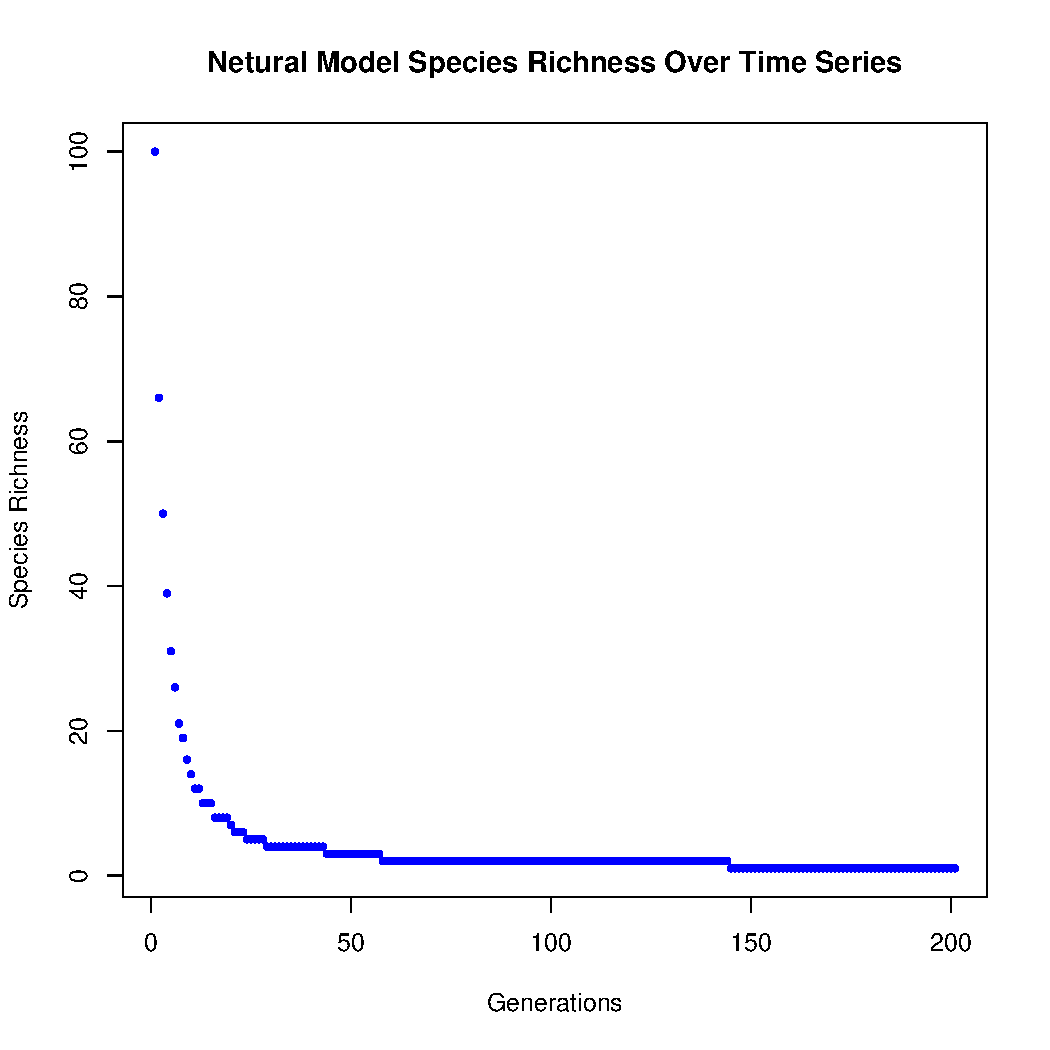
\includegraphics[width = 0.6\hsize]{../../results/Question8.pdf} 
\caption{Netural model species richness over time series}
As time flows, the species richness started from 100 will finally decline to 1.
\end{figure}

Q: What state will the system always converge to if you wait long enough?  Why is this?

A: If wait long enough, there will be only one species converge to the community, because the model does not incorporate any opportunity for
diversity to be increased, no speciation or mutation, as generations progress and individuals die and extinct (there are only one individual per species, which makes it easy to extinct and that why the richness decrease so fast) in the community, the species that replace it tends to become more frequent in the population, thus more favorable in future random replacement, finally dominate the community.


\subsection{Question 12}
Perform a neutral theory simulation with speciation and plot species richness against time. Plot two time series on the same axes in different colours showing how the simulation progresses from two different initial states given by initialise\_max and initialise\_min.

\begin{figure}[!ht]
\centering 
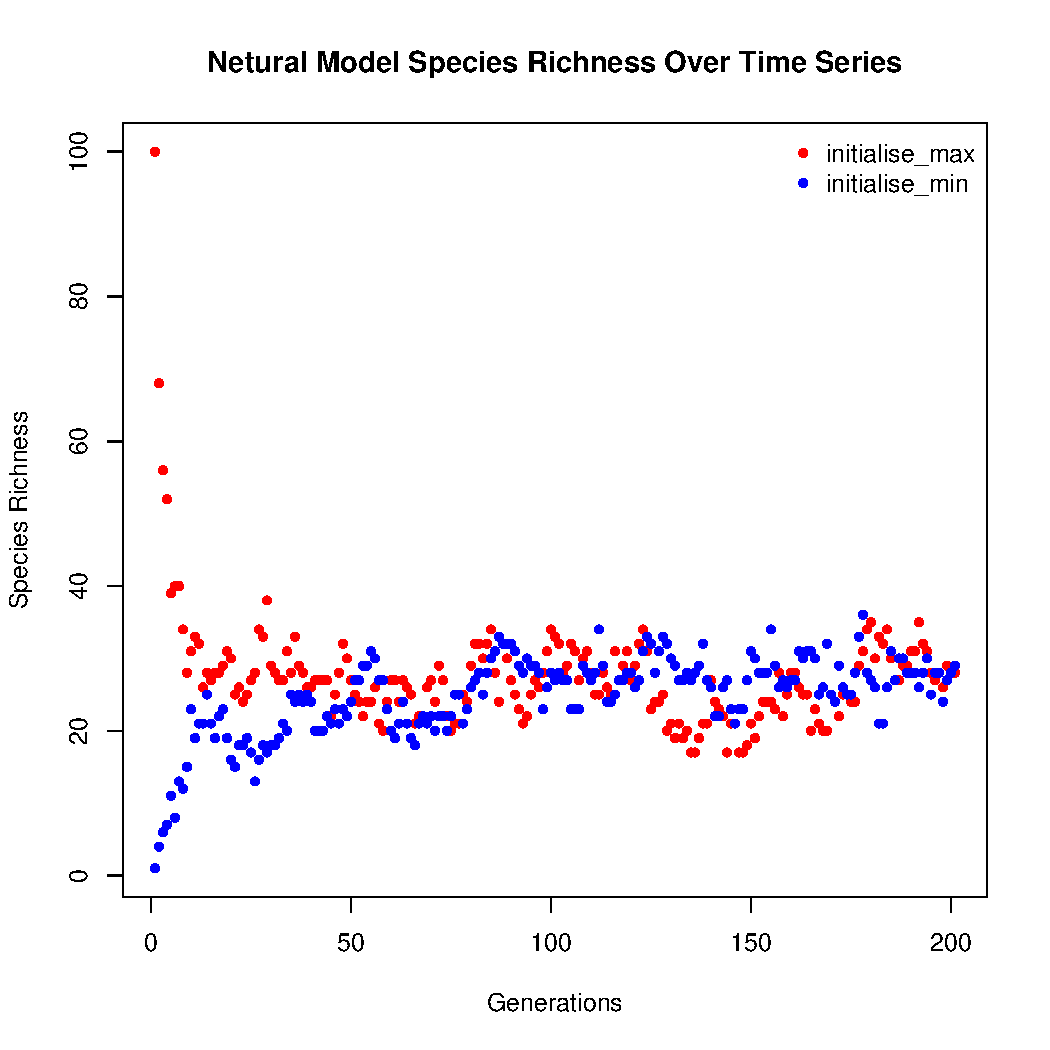
\includegraphics[width = 0.6\hsize]{../../results/Question12.pdf} 
\caption{Netural model species richness over time series with speciation}
As time flows, the species richness started from initialise\_max and initialise\_min will finally fluctuate roughly between 20 and 30.
\end{figure}

Q: Explain what you found from this plot about the effect of initial conditions. Why does the neutral model simulation give you those particular results?

A: We can easily find that both initial conditions converge to the same values (roughly 25) of species richness in a very similar number of time steps (around 25 generations). Therefore, demonstrates that the initial conditions have no discernible impact on the outcome of this neutral model. By adjusting the parameters we know that the speed and value of convergence are determined by the size of community and speciation rate. This is because new species are constantly arising in the population, and eventually, the likelihood of removing a species (extinction) equals the likelihood of creating a new species (immigration/speciation), and for this graph, the balance fluctuates between 20 to 30. So giving a specific size of community and speciation rate, wait long enough will lead to a species balance.



\subsection{Question 16}
Run a neutral model simulation using the same parameters as in question 12 for a ‘burn in’ period of 200 generations. Next record the species abundance octave vector. Then repeatedly continue the simulation for a further 2000 generations, and record the species abundance octave vector every 20 generations.

\begin{figure}[!ht]
\centering 
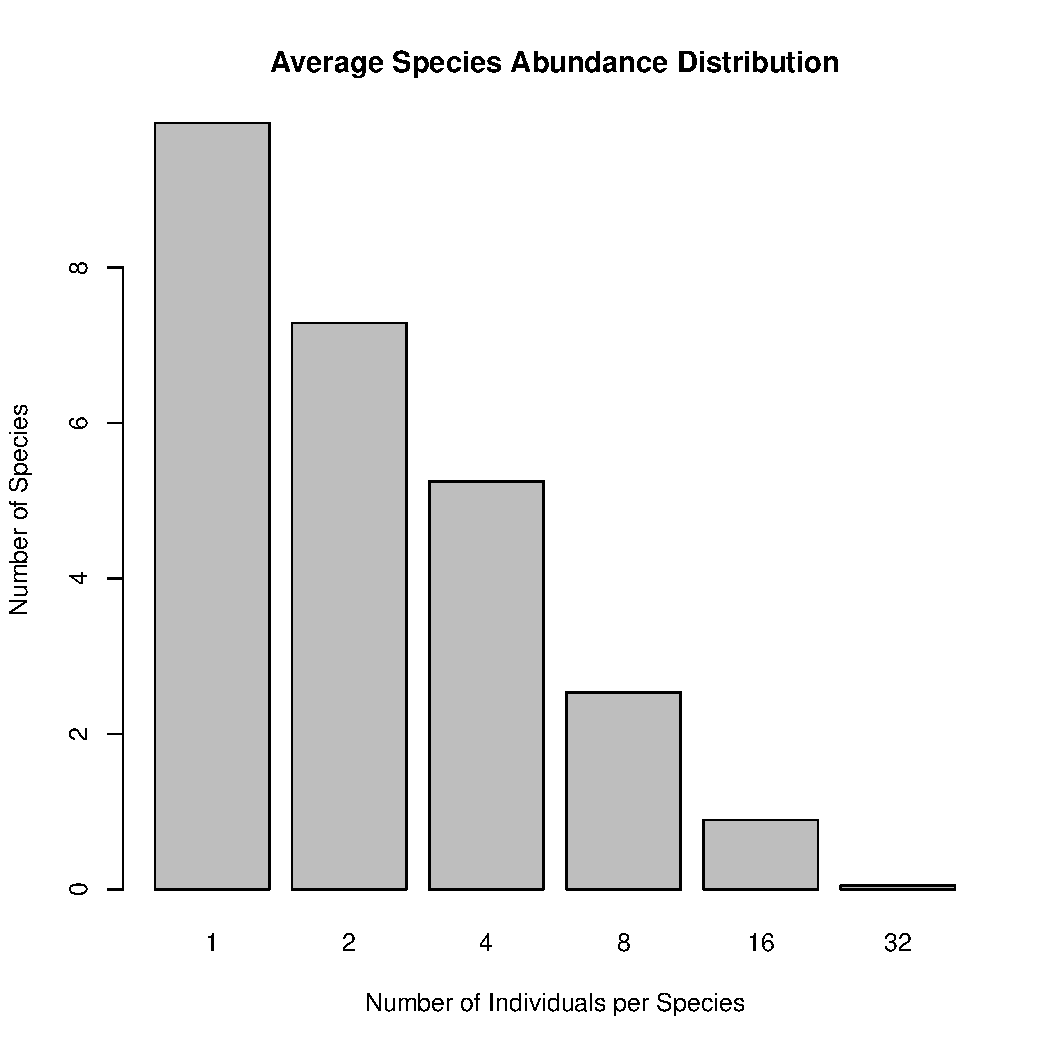
\includegraphics[width = 0.6\hsize]{../../results/Question16.pdf} 
\caption{Average Species Abundance Distribution}
The x-axis number is the exponent of 2, representing the starting value of the statistical abundance. The number of species with more individuals is decreasing. Like a normal distribution。
\end{figure}

Q: Does the initial condition of the system matter?  Why is this?

A: Basically No. As we discussed in question 12, a ‘burn in’ period of 200 generations is long enough to make it converge, and the converged value is determined by the size of community and speciation rate. If a shorter burn in a period was used, then a bigger difference would be seen as it takes time for the impact of the initial conditions to be negligible, especially if extreme conditions were used.


\subsection{Challenge A}
Plot the mean species richness as a function of time (measured in simulation steps) across a large number of repeat simulations using the same parameters as in question 16.  Add a 97.2\% confidence interval on the species richness at each point in time.  Repeat this for both initial conditions (high initial diversity and low initial diversity). Estimate the number of time steps needed for the system to reach dynamic equilibrium.

\begin{figure}[!ht]
\centering 
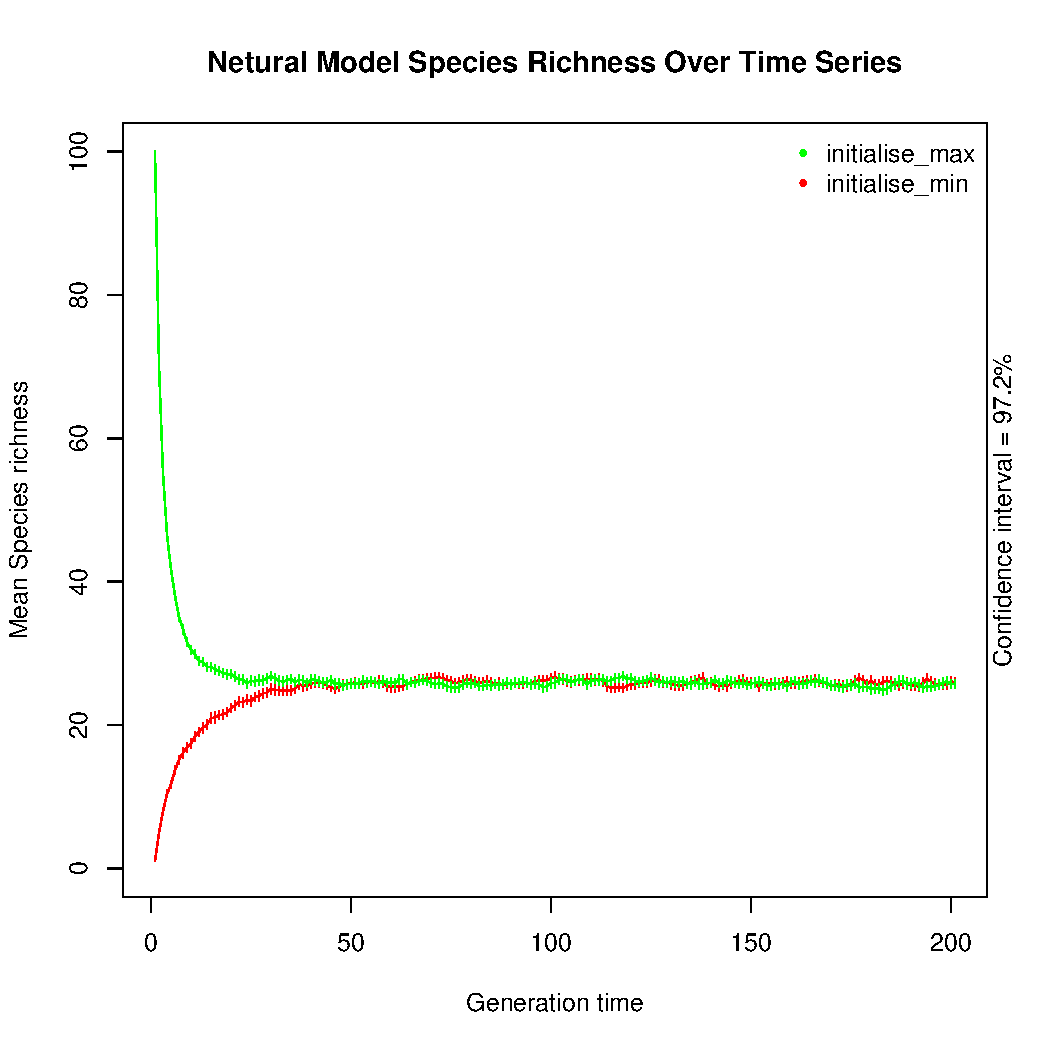
\includegraphics[width = 0.6\hsize]{../../results/ChallengeA.pdf} 
\caption{Netural model average species richness over time series}
Graph shows mean species richness over time, with two initial conditions, max and min diversity. The vertical lines show the 97.2\% confidence intervals of both conditions. The number of time steps required for dynamic equilibrium to be reached is roughly 40 generations. This is true for starting communities of either maximum or minimum richness.
\end{figure}




\subsection{Challenge B}
Plot a graph showing many averaged time series for a whole range of different initial species richnesses. In each initial community state, each individual should be equally likely to take any species identity.

\begin{figure}[!ht]
\centering 
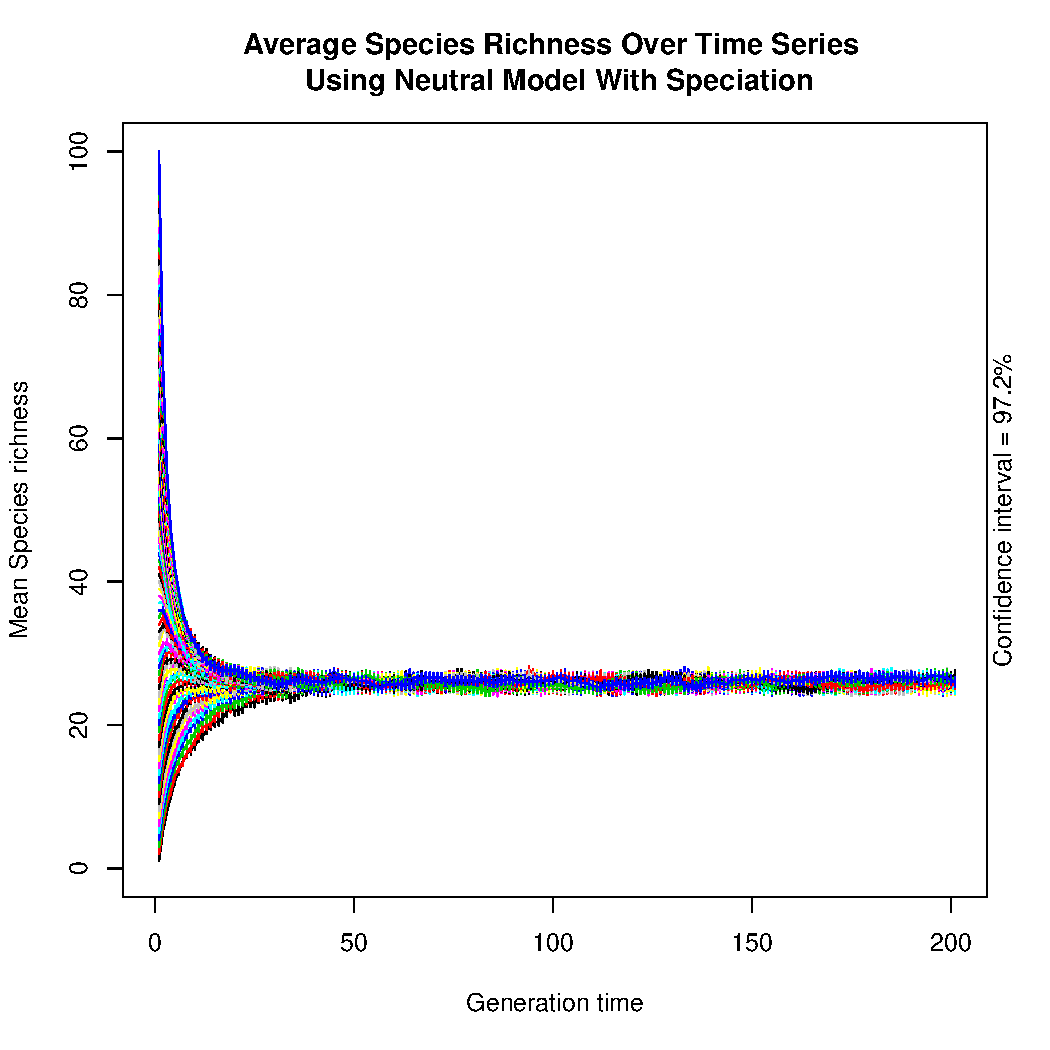
\includegraphics[width = 0.6\hsize]{../../results/ChallengeB.pdf} 
\caption{Averaged species richness through time for
a variety of initial species richness values}
Graph shows mean species richness over time, with many initial conditions. The vertical lines show the 97.2\% confidence intervals. 
\end{figure}

\newpage
\section{Simulations using HPC}
\subsection{Question 20}
Provide four bar graphs in a multi-panel graph (one for each simulation size) each showing a mean species abundance octave result from all simulation runs of that size. Only use data of the abundance octaves after the burn in time is up.

\begin{figure}[!ht]
\centering 
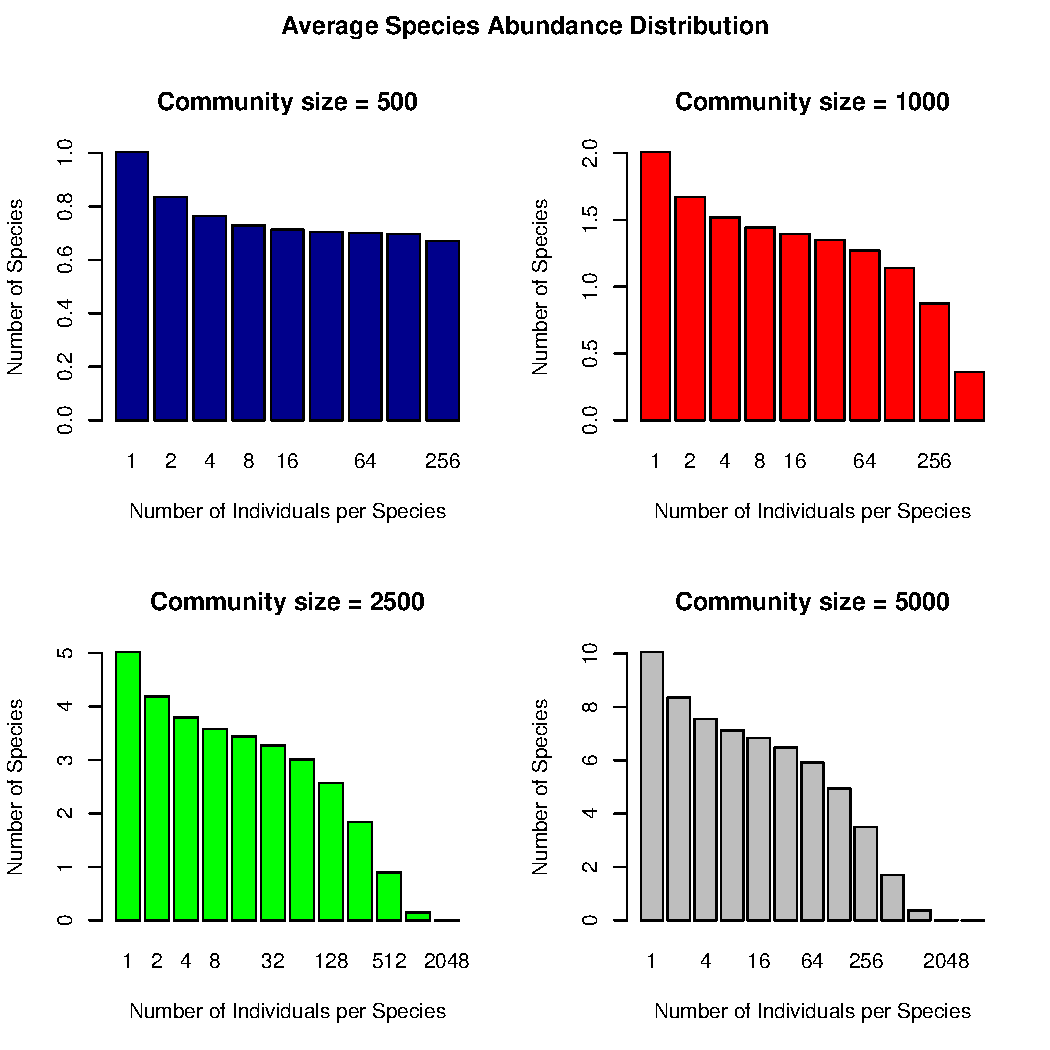
\includegraphics[width = 0.8\hsize]{../../results/Question20.pdf} 
\caption{Mean species abundance octaves for community sizes of 500, 1000, 2500 and 5000 following burn-in period}
The x-axis number is the exponent of 2, representing the starting value of the statistical abundance.
\end{figure}


\subsection{Challenge C}
Plot a graph of mean species richness against simulation generation and use it to inform you more precisely how long should have been allowed as a burn in period for different values of J.

\begin{figure}[htbp]
\centering
\begin{minipage}[t]{0.48\textwidth}
\centering
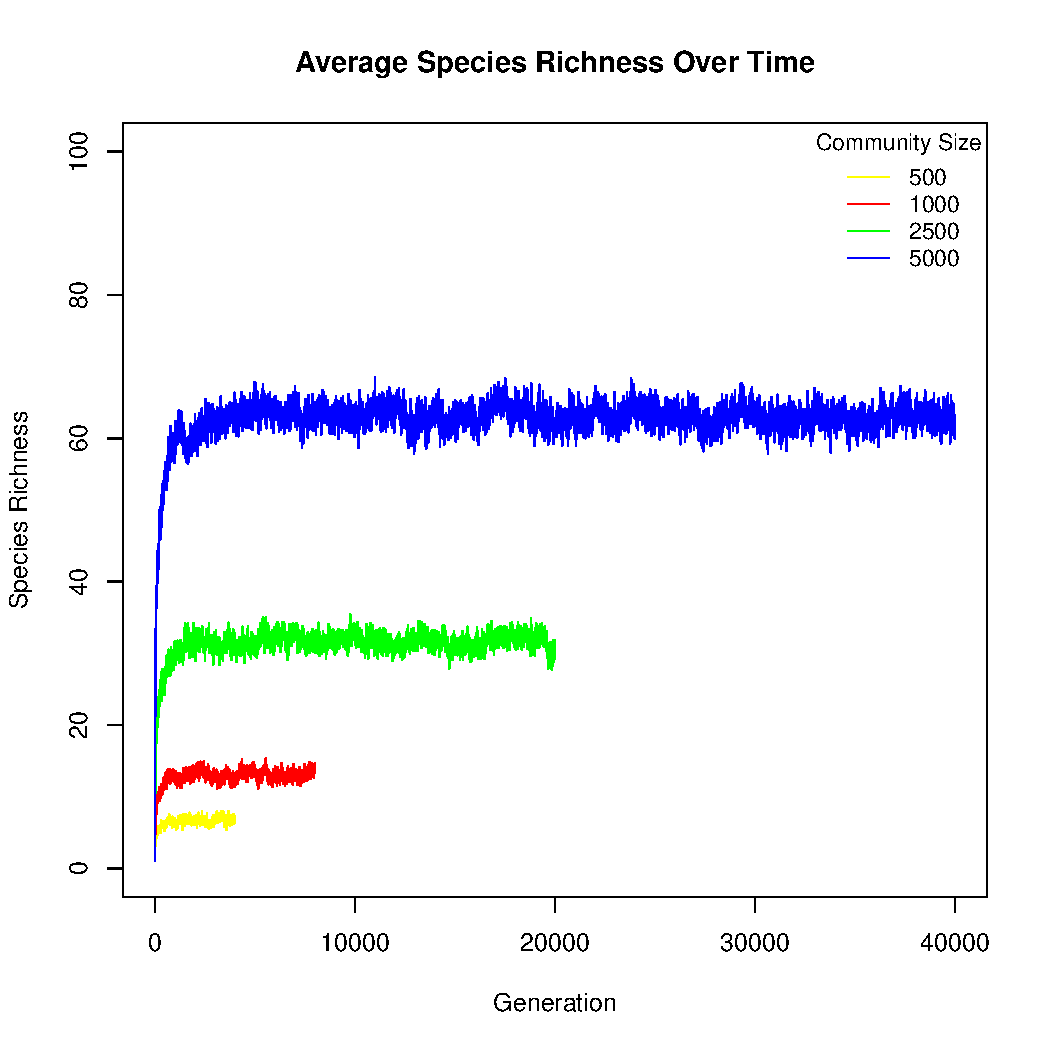
\includegraphics[width=6.7cm]{../../results/ChallengeC.pdf}
\caption{Whole Vision}
\end{minipage}
\begin{minipage}[t]{0.48\textwidth}
\centering
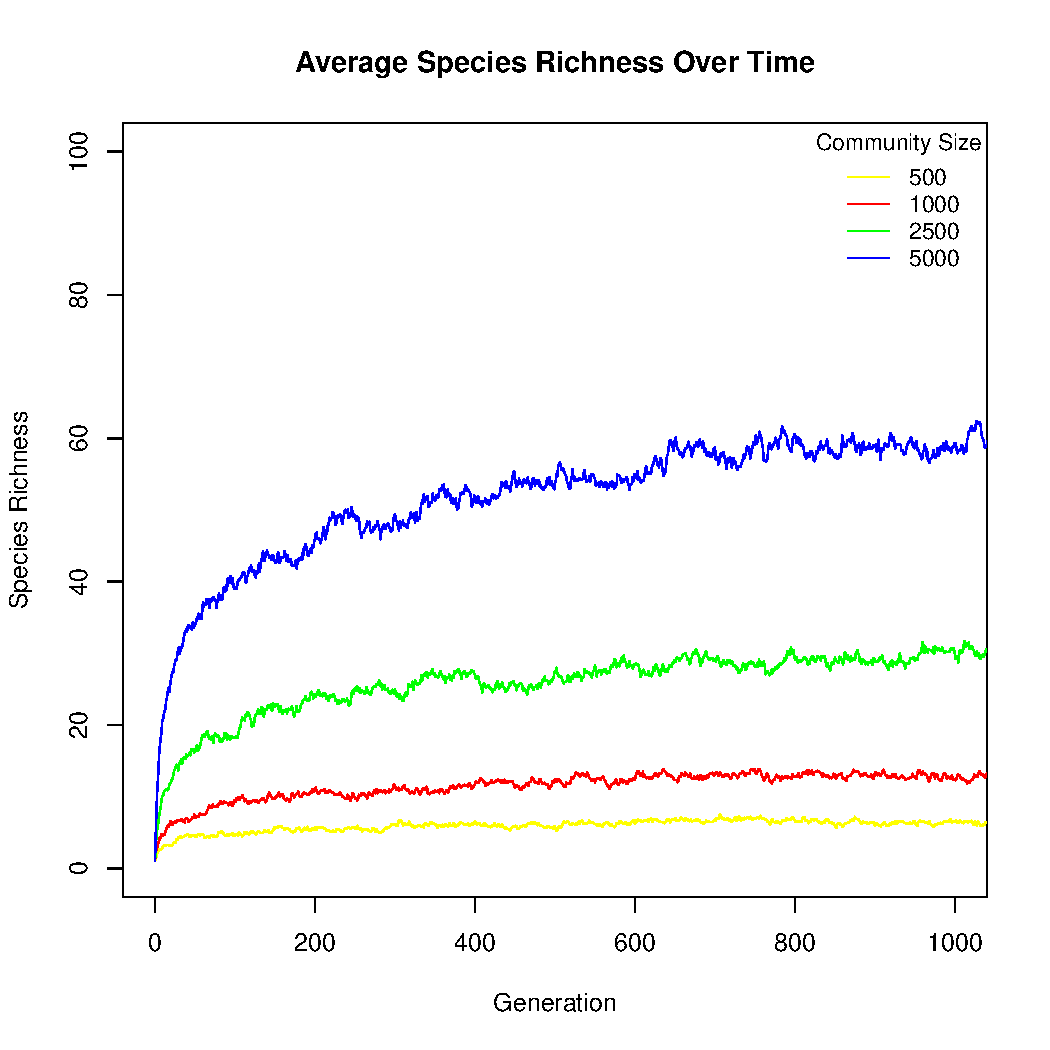
\includegraphics[width=6.7cm]{../../results/ChallengeC-2.pdf}
\caption{Zoom in Vision}
\end{minipage}
\end{figure}

From looking at both the graphs, it appears that for community sizes of 500, 1000, 2500 and 5000 equilibrium have been reached by around 50, 200, 400 and 600 generations. This suggests that a burn-in period of 8 times the community size, as used in our simulations, is excessive.

\newpage
\subsection{Challenge D}
Conduct further simulations of the same system using coalescence 

\begin{figure}[!ht]
\centering 
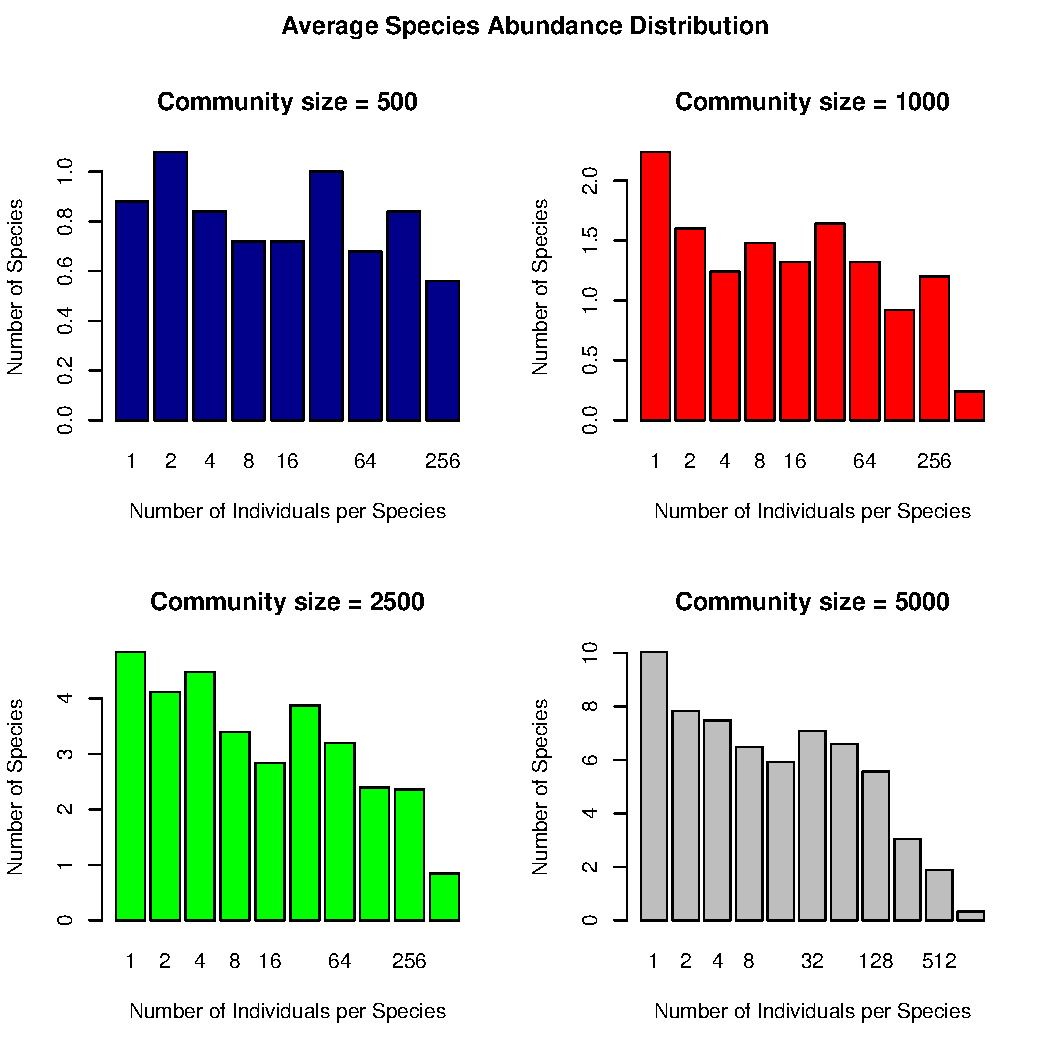
\includegraphics[width = 0.8\hsize]{../../results/ChallengeD.pdf} 
\caption{Mean species abundance octaves for community sizes of 500, 1000, 2500 and 5000 using coalescence}
The x-axis number is the exponent of 2, representing the starting value of the statistical abundance.
\end{figure}

From observing Figure 6 and Figure 9. It might have some slight differences, but theoretically, we can assume that the neutral simulation run on the HPC cluster and the coalescence model return qualitatively similar results with regards to average species abundance distributions. 

As for the time spent, coalescence model spent around 5-6 seconds, while time series model using cluster require 4140001.822 seconds, which is over 7 hundred thousand times as much CPU time as that taken by the coalescence simulations. It's really amazing, and maybe this is the power of the algorithm.

The reason why the coalescence simulations were so much faster is that, firstly, the algorithm takes a reverse thinking, only lineages that actually appear in the sample are considered and tracked back in time. This contrasts to the forward based model in which many lineages simulated are eventually doomed for extinction meaning that the time taken to simulate these is effectively wasted if you only analyse a community from a particular time point at which these lineages are not present. This is also more in line with our ecological analysis method, analysis from the existing sample. Another important reason is that the forward time series simulation requires a burn-in period which allows the community to reach a dynamic equilibrium. It is not required when using coalescence as when a single lineage is left it is known that the community was at equilibrium.

So it comes back to the advantages and disadvantages of coalescence. The advantages are that It is always at equilibrium, and sampling based, which makes it faster. But it is not ideal for time series, complex to program and be understood, and has fewer ways in which model can be changed than the forward time series model.

\newpage
\section{Fractals in nature}
\subsection{Question 21}
What are the fractal dimensions of these objects?  Show and briefly explain your workings.

\begin{figure}[htbp]
\centering
\begin{minipage}[t]{0.48\textwidth}
\centering

\includegraphics[width=5.7cm,height=5.7cm]{./1.png}
\end{minipage}
\begin{minipage}[t]{0.48\textwidth}
\centering
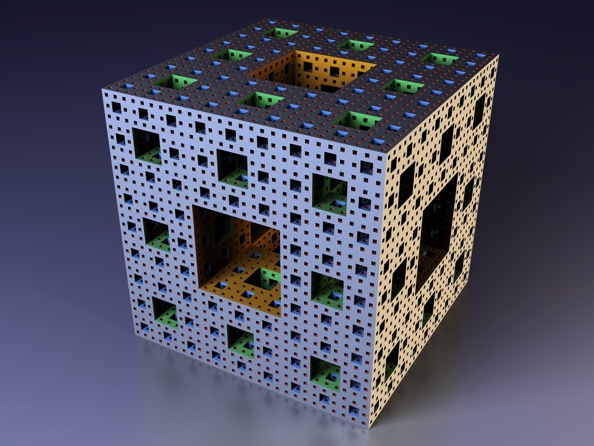
\includegraphics[width=6.7cm,height=5.7cm]{./2.jpg}
\end{minipage}
\end{figure}
For the object above-left, it is clear that tripling the width of the object requires 8 times as many of the original to reconstruct a larger, self-similar version of the image. As such, $$D = \frac{\log(8)}{\log(3)} = 1.893.$$

Similarly, tripling the width requires 20 times as many objects. $$D = \frac{\log(20)}{\log(3)} = 2.727.$$

\newpage
\subsection{Challenge E}
Try starting the chaos game from a completely different initial position X what happens now and why? Try starting with the points of an equilateral triangle as A , B and C to produce a classic Sierpinski Gasket.


\begin{figure}[htbp] 
\centering 
\subfigure[Initial X at (1,4)]{ 
\begin{minipage}[t]{0.48\textwidth} 
\centering 
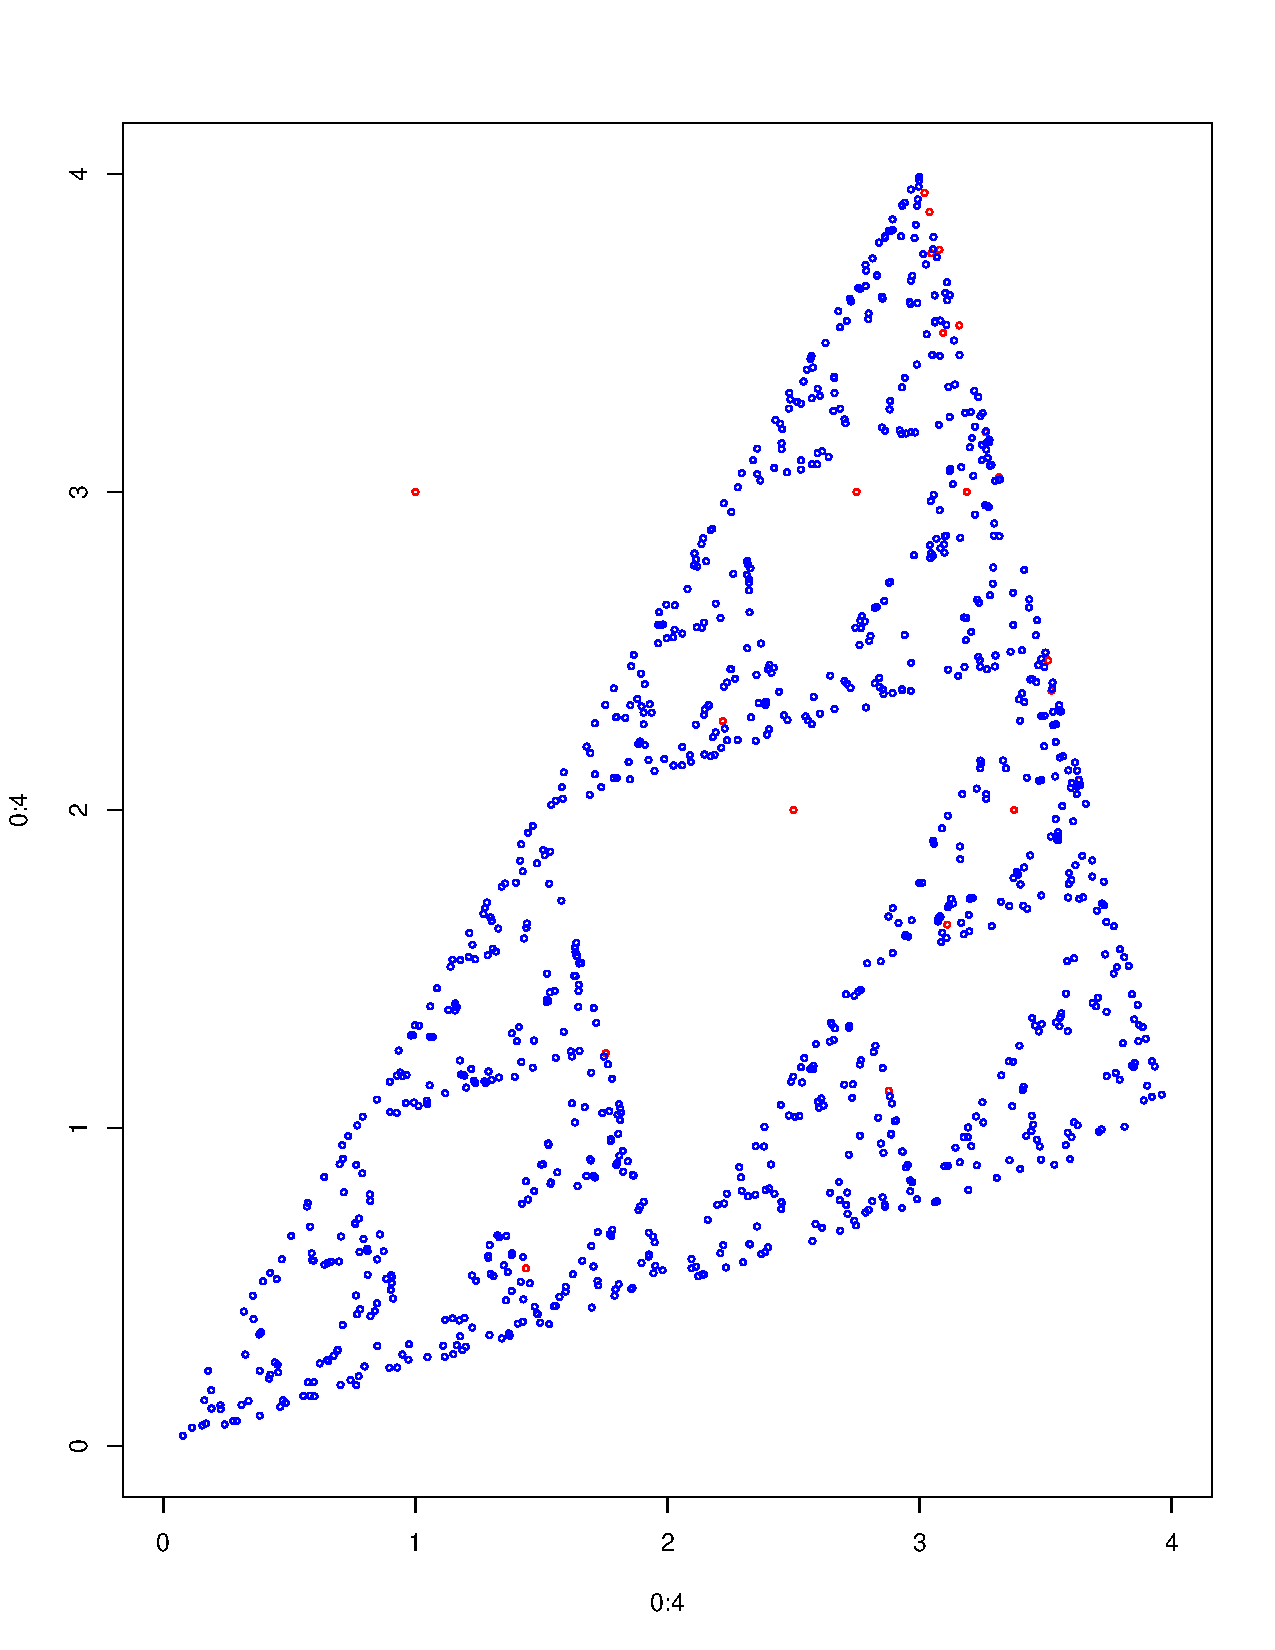
\includegraphics[width=6.7cm,height=4.7cm]{../../results/Gasket1.pdf} 
\end{minipage}%
}%
\subfigure[Initial X at (2,1)]{ 
\begin{minipage}[t]{0.48\textwidth} 
\centering 
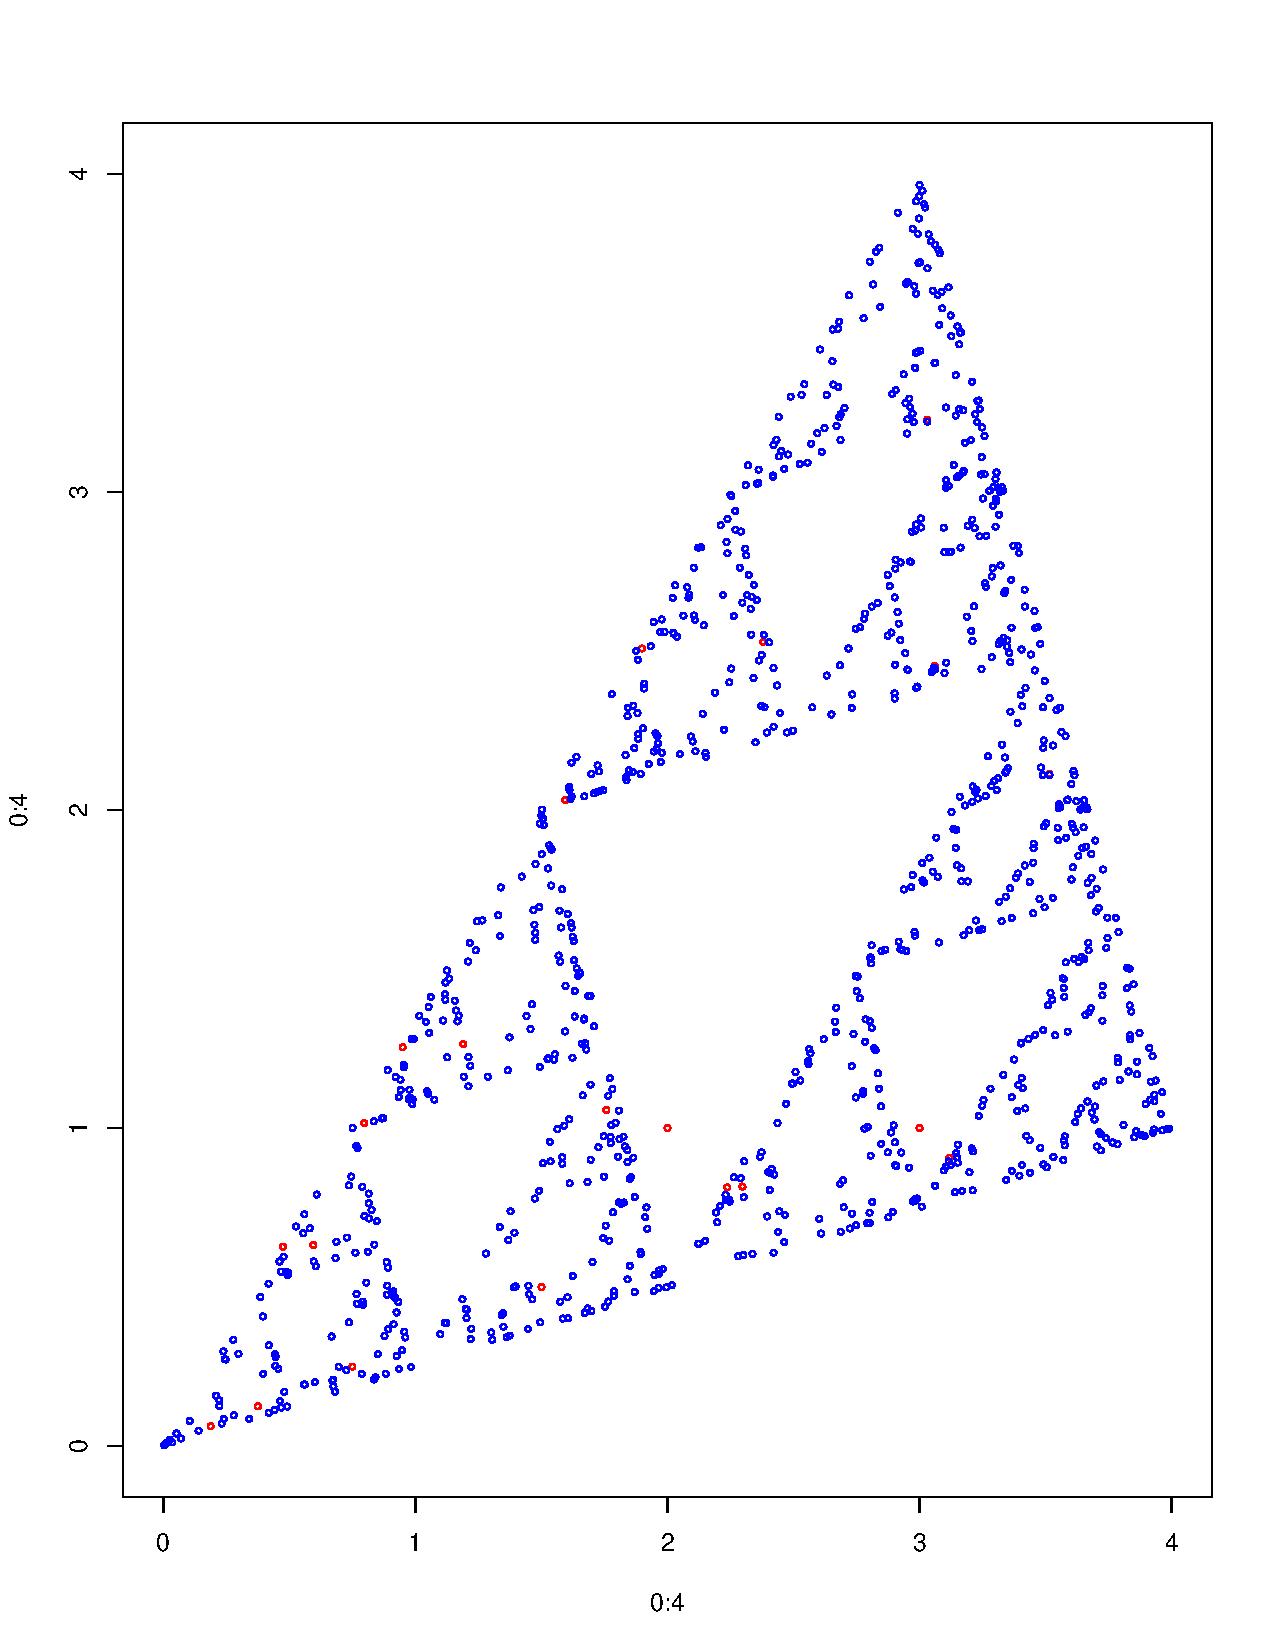
\includegraphics[width=6.7cm,height=4.7cm]{../../results/Gasket2.pdf} 
\end{minipage}
}
\centering 
\caption{Starting the chaos game from a completely different initial position}

\begin{minipage}[t]{0.48\textwidth}
\centering
\includegraphics[width=6.7cm,height=4.7cm]{../../results/Gasket3.pdf}
\caption{Classic Sierpinski Gasket}
\end{minipage}
\begin{minipage}[t]{0.48\textwidth}
\centering
\includegraphics[width=6.7cm,height=4.7cm]{../../results/Gasket4.pdf}
\caption{fun chaos\_game}
\end{minipage}

\end{figure}

As we can see above, whether X it is initialized in the blank area inside the triangle or externally,after a certain step (mark with a red dot), eventually, it will infinitely close to the three vertices of a triangle, and then form a Sierpinski Gasket.


\subsection{Challenge F}
As the line size limit gets smaller, the fractals take longer to generate, but are more detailed.


\begin{figure}[htbp] 
\centering 
\subfigure[Use rainbow colours]{ 
\begin{minipage}[t]{0.32\textwidth} 
\centering 
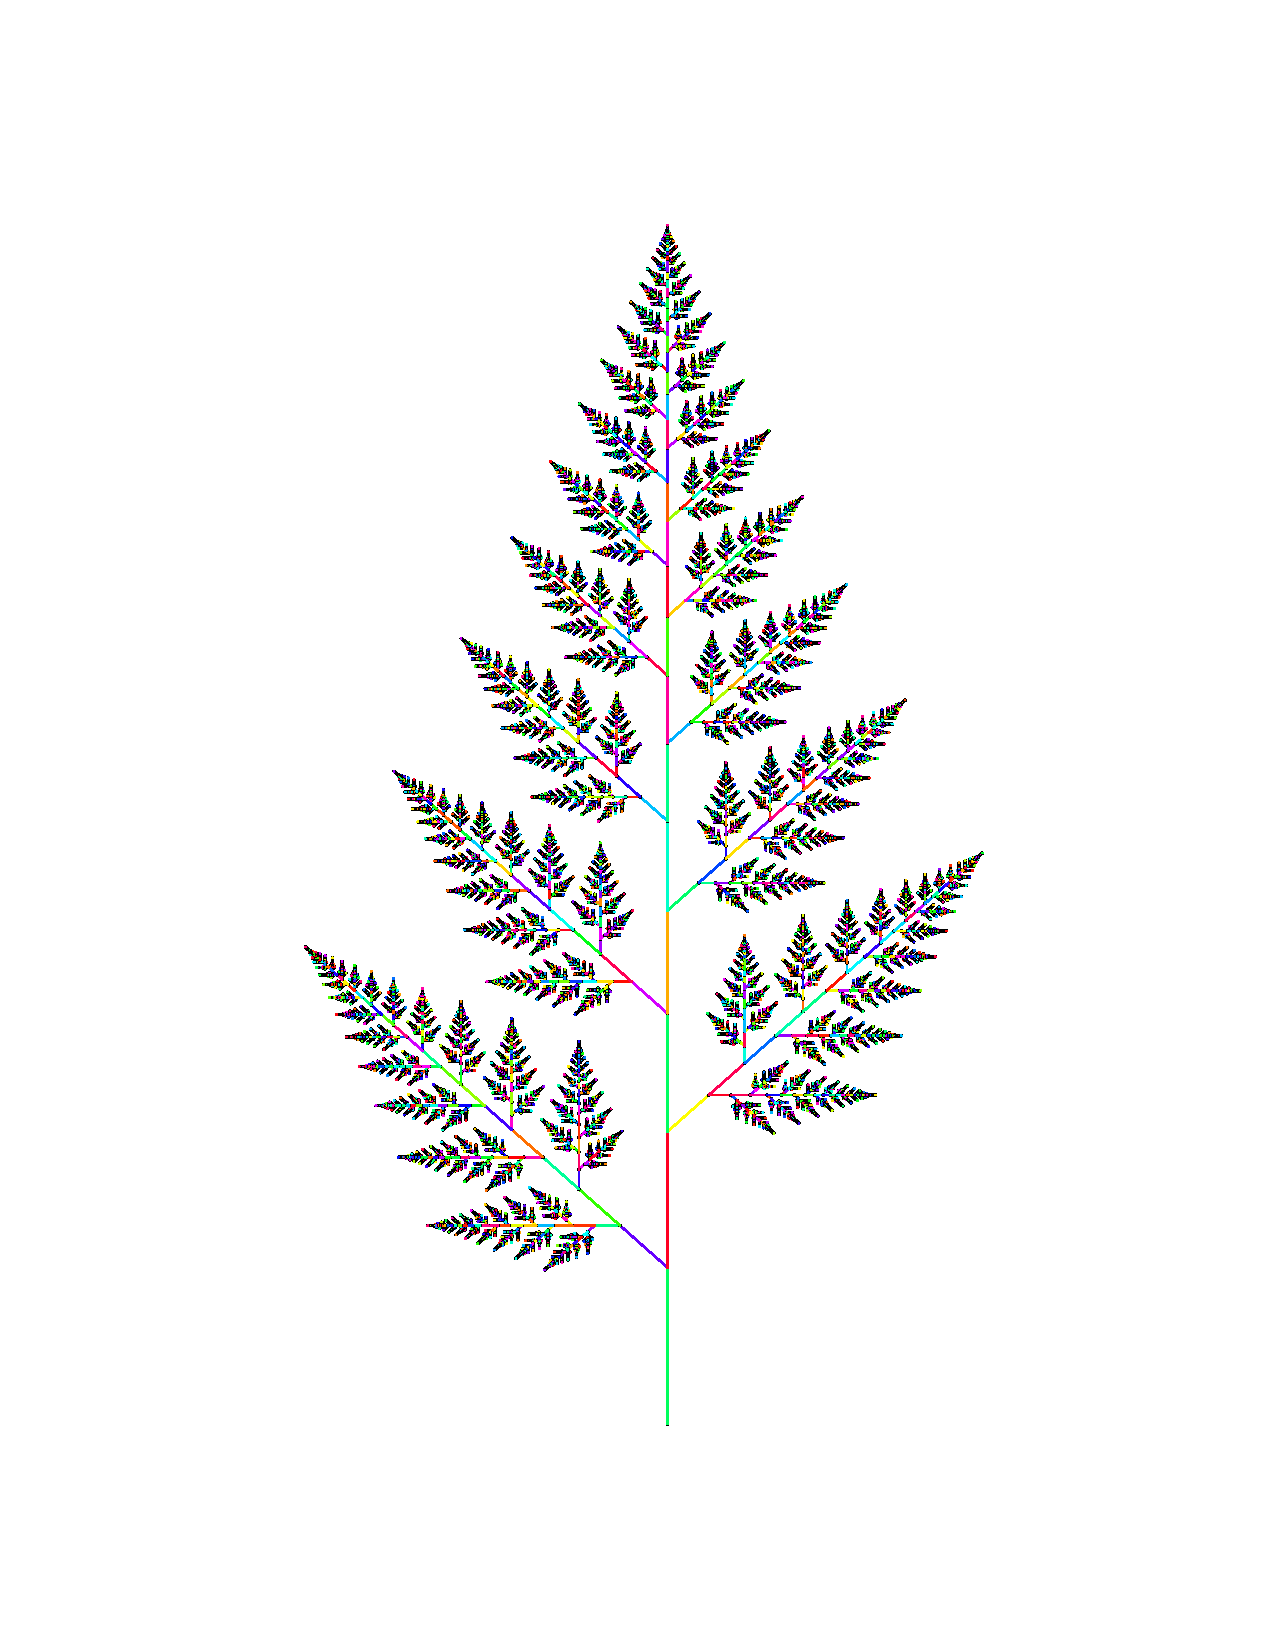
\includegraphics[width=4.5cm,height=4.7cm]{../../results/fern1.pdf} 
\end{minipage}%
}%
\subfigure[Adjust the angle]{ 
\begin{minipage}[t]{0.32\textwidth} 
\centering 
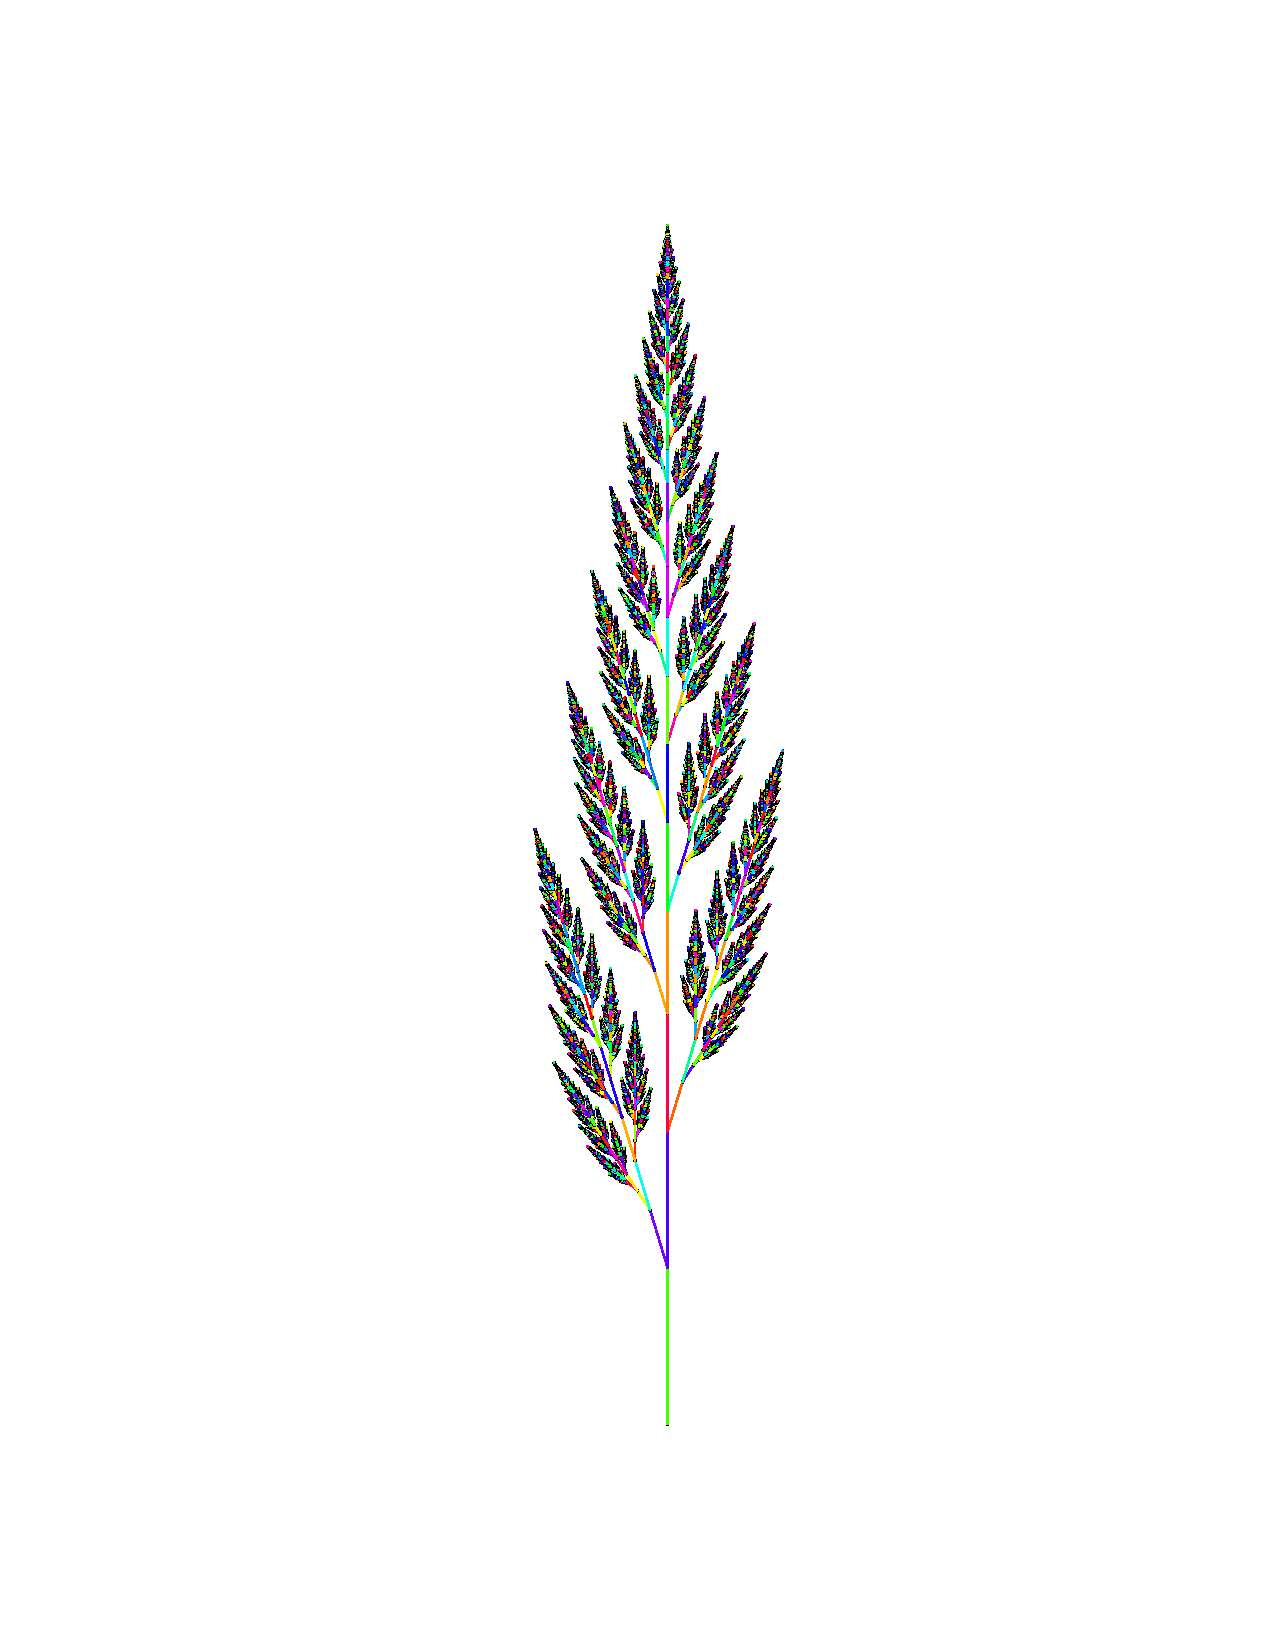
\includegraphics[width=4.5cm,height=4.7cm]{../../results/fern2.pdf} 
\end{minipage}%
}%
\subfigure[Adjust length change]{ 
\begin{minipage}[t]{0.32\textwidth} 
\centering 
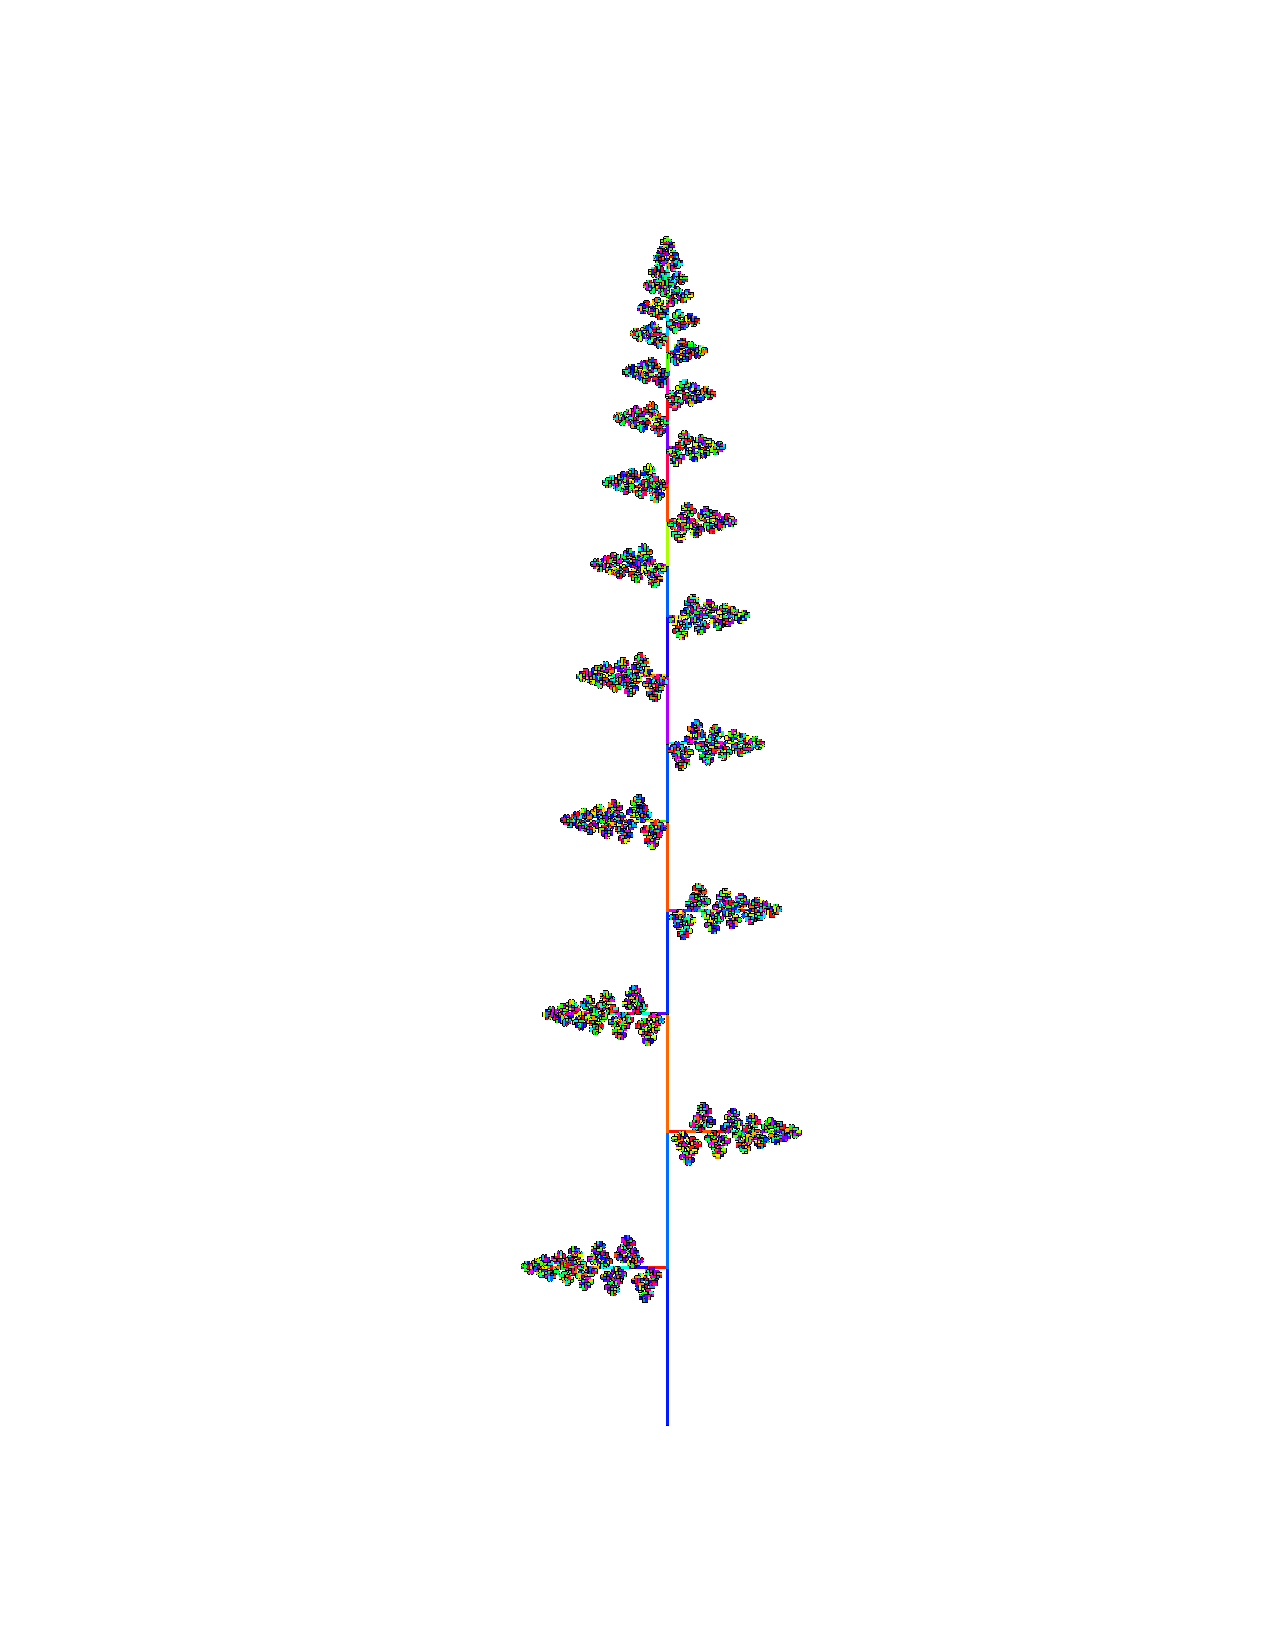
\includegraphics[width=4.5cm,height=4.7cm]{../../results/fern3.pdf} 
\end{minipage}
}
\centering 
\caption{Challenge F creation}
\end{figure}


\subsection{Challenge F}

Challenge\_G$<$-function(s=c(3,0),d=pi/2,l=1,r=1,v=segments,o=cos,i=sin,

p=plot(c(0,6),c(0,8),"n"),j=f(s,d,l,r),a=0.38,b=0.87,k=0.007,z=pi/4)

\{p;f=function(s,d,l,r)\{e=c(s[1]+l*o(d),s[2]+l*i(d));v(s[1],s[2],e[1],e[2]);

if(l$>$k)\{f(e,d+r*z,l*a,r);f(e,d,l*b,-r\}\};j\}


\lstset{ numbers=left, 
numberstyle= \tiny, 
keywordstyle= \color{ blue!70}, 
commentstyle= \color{red!50!green!50!blue!50}, frame=shadowbox, 
rulesepcolor= \color{ red!20!green!20!blue!20} , escapeinside=``, 
language=R
} 
\centering 
\begin{lstlisting} 
Challenge_G <- function(s=c(2,0),d=pi/2,l=1,r=1){
    plot(c(0,4),c(0,8),"n")
    f <- function(s,d,l,r){
        e=c(s[1]+l*cos(d),s[2]+l*sin(d))
        lines(c(s[1],e[1]),c(s[2],e[2]))
        if(l>.007){
        f(e,d+r*pi/4,l*.38,r)
        f(e,d,l*.87,-r)}
    }
    f(s,d,l,r)
} 

\end{lstlisting}

\end{document}